\documentclass[10pt, svgnames, compress, red]{beamer}
\usepackage{lmodern}
\usepackage{palatino}
\usepackage[T1]{fontenc}
\usepackage[utf8]{inputenc}
\usepackage[french]{babel}

%%%%%%%%%%%%%%%%%%%%%%%%%%%%%%%%%%%%%%%%%%%%%%%%%%%%%%%%%%%%%%%%%%%%%%%%%%%%%%%%%%%%%%%%%%%%%%%%%%%%%%%%%%%%%%
% PACKAGES
%%%%%%%%%%%%%%%%%%%%%%%%%%%%%%%%%%%%%%%%%%%%%%%%%%%%%%%%%%%%%%%%%%%%%%%%%%%%%%%%%%%%%%%%%%%%%%%%%%%%%%%%%%%%%%

\usepackage{multimedia}				% to use multimedia
\usepackage{graphicx}				  % to use graphics
\usepackage{subfigure}				% to use figure in figure
\hypersetup{pdfstartview={Fit}}
\graphicspath{{./images/}}		% to say where are image
\usepackage{natbib}
\usepackage{caption}
\usepackage{appendixnumberbeamer}
\usepackage{listings}

% \RequirePackage{pageGardeEnsta}
% \usepackage[svgnames]{xcolor}

%%%%%%%%%%%%%%%%%%%%%%%%%%%%%%%%%%%%%%%%%%%%%%%%%%%%%%%%%%%%%%%%%%%%%%%%%%%%%%%%%%%%%%%%%%%%%%%%%%%%%%%%%%%%%%
% THEME
%%%%%%%%%%%%%%%%%%%%%%%%%%%%%%%%%%%%%%%%%%%%%%%%%%%%%%%%%%%%%%%%%%%%%%%%%%%%%%%%%%%%%%%%%%%%%%%%%%%%%%%%%%%%%%
\mode<presentation>
\usetheme{Warsaw}
\usecolortheme{lily}
\useoutertheme[subsection=false]{smoothbars}
\useinnertheme{circles}
\useoutertheme{shadow}
\usefonttheme{serif}

%%%%%%%%%%%%%%%%%%%%%%%%%
\hypersetup{
  pdfpagemode = FullScreen,% afficher le pdf en plein écran
  pdfkeywords = {},%
  pdfcreator  = {PDFLaTeX},%
  pdfproducer = {PDFLaTeX}%
}




%%%%%%%%%%%%%%%%%%%%%%%%%%%%%%%%%%%%%%%%%%%%%%%%%%%%%%%%%%%%%%%%%%%%%%%%%%%%%%%%%%%%%%%%%%%%%%%%%%%%%%%%%%%%%%
% CONFIGURATION
%%%%%%%%%%%%%%%%%%%%%%%%%%%%%%%%%%%%%%%%%%%%%%%%%%%%%%%%%%%%%%%%%%%%%%%%%%%%%%%%%%%%%%%%%%%%%%%%%%%%%%%%%%%%%%

\usepackage{enumitem}
\newcounter{th}[section]

\newcommand{\definitionn}[2]{\noindent\fcolorbox{OliveDrab}{white}{\stepcounter{th}
    \parbox{\textwidth}{\textbf{\textcolor{OliveDrab}{Definition~\thesection.\theth~:}}{~
        \textit{#1}}~\setlength{\parindent}{15pt}\par#2\par}}\par~\\}


\lstdefinelanguage{suricata}
{morekeywords= {alert, tcp, http, tls, ip, ipv4, ipv4, drop, pass, sid, priority, rev, classtype, threshold, metadata, reference, tag, msg, content, uricontent, pcre, ack, seq, depth, distance, within, offset, replace, nocase, fast\_pattern, rawbytes, byte\_test, byte\_jump, sameip, ip\_proto, flow, window, ftpbounce, isdataat, id, rpc, dsize, flowvar, flowint, pktvar, noalert, flowbits, stream\_size, ttl, itype, icode, tos, icmp\_id, icmp\_seq, detection\_filter, ipopts, flags, fragbits, fragoffset, gid, nfq\_set\_mark, tls.version, tls.subject, tls.issuerdn, tls.fingerprint, tls.store, http\_cookie, http\_method, urilen, http\_client\_body, http\_server\_body, http\_header, http\_raw\_header, http\_uri, http\_raw\_uri, http\_stat\_msg, http\_stat\_code, http\_user\_agent, ssh.protoversion, ssh.softwareversion, ssl\_version, ssl\_state, byte\_extract, file\_data, dce\_iface, dce\_opnum, dce\_stub\_data, asn1, filename, fileext, filestore, filemagic, filemd5, filesize, l3\_proto, luajit},
otherkeywords={ipv4-csum, tcpv4-csum, tcpv6-csum, udpv4-csum, udpv6-csum, icmpv4-csum, icmpv6-csum, decode-event, app-layer-event, engine-event, stream-event},
sensitive=true,
morecomment=[l]{//},
morecomment=[s]{/*}{*/},
morestring=\color{blue}[b]",
keywordstyle=\bfseries\color{red!70!black},
}




% Permet la non numérotation des pages en annexes pour réaliser des slides cachés
\expandafter\def\expandafter\insertshorttitle\expandafter{%
  \insertshorttitle\hfill\insertframenumber\,/\,\inserttotalframenumber}

%%%% Permet affiche en début de chaque section, les noms de sections et
%%%% noms de sous-sections de la section en cours.
\AtBeginSection[]{
  \begin{frame}
    \begin{center}{\Large Sommaire }\end{center}
    \tableofcontents[currentsection,hideothersubsections]
    \transdissolve[duration=0.1]
  \end{frame}

}

% POUR CONFIGURER LE FOND
\setbeamercolor{background canvas}{bg=Beige}

% POUR CONFIGURER LA LIGNE DU BAS ET HAUT
\setbeamertemplate{footline}{
\leavevmode%
\hbox{\hspace*{-0.06cm}
\begin{beamercolorbox}[wd=.2\paperwidth,ht=2.25ex,dp=1ex,center]{author in head/foot}%
	\usebeamerfont{author in head/foot}\insertshortauthor%~~(\insertshortinstitute)
\end{beamercolorbox}%
\begin{beamercolorbox}[wd=.6\paperwidth,ht=2.25ex,dp=1ex,center]{section in head/foot}%
	\usebeamerfont{section in head/foot}\insertshorttitle
\end{beamercolorbox}%
\begin{beamercolorbox}[wd=.2\paperwidth,ht=2.25ex,dp=1ex,right]{section in head/foot}%
	\usebeamerfont{section in head/foot}\insertshortdate{}\hspace*{2em}
	\insertframenumber{} / \inserttotalframenumber\hspace*{2ex}
\end{beamercolorbox}}%
\vskip0pt%
}
\bibliographystyle{plain}
% make bibliography entries smaller
\renewcommand*{\bibfont}{\footnotesize}
% If you have more than one page of references, you want to tell beamer
% to put the continuation section label from the second slide onwards
\setbeamertemplate{frametitle continuation}[from second]
% Now get rid of all the colours
\setbeamercolor*{bibliography entry title}{fg=black}
\setbeamercolor*{bibliography entry author}{fg=black}
\setbeamercolor*{bibliography entry location}{fg=black}
\setbeamercolor*{bibliography entry note}{fg=black}
% and kill the abominable icon
\setbeamertemplate{bibliography item}{}


%%%%%%%%%%%%%%%%%%%%%%%%%%%%%%%%%%%%%%%%%%%%%%%%%%%%%%%%%%%%%%%%%%%%%%%%%%%%%%%%%%%%%%%%%%%%%%%%%%%%%%%%%%%%%%
% TITRE
%%%%%%%%%%%%%%%%%%%%%%%%%%%%%%%%%%%%%%%%%%%%%%%%%%%%%%%%%%%%%%%%%%%%%%%%%%%%%%%%%%%%%%%%%%%%%%%%%%%%%%%%%%%%%%

\institute{ENSTA Bretagne}
\title{Sniff Hynesim}
\subtitle{}
\subject{}
\author{IETA RIGAUD Michaël}
\logo{
\includegraphics[scale=0.1]{logo_ENSTA_Bretagne_Vertical_CMJN}}

%%%%%%%%%%%%%%%%%%%%%%%%%%%%%%%%%%%%%%%%%%%%%%%%%%%%%%%%%%%%%%%%%%%%%%%%%%%%%%%%%%%%%%%%%%%%%%%%%%%%%%%%%%%%%%
% DOCUMENT
%%%%%%%%%%%%%%%%%%%%%%%%%%%%%%%%%%%%%%%%%%%%%%%%%%%%%%%%%%%%%%%%%%%%%%%%%%%%%%%%%%%%%%%%%%%%%%%%%%%%%%%%%%%%%%

\begin{document}
\begin{frame}
  \titlepage
  % \includegraphics[height=1.2cm]{Image22.png}
  \transdissolve[duration=0.1]
\end{frame}


\section{Introduction}
\begin{frame}
  \frametitle{Introduction}
  \begin{figure}[h]
    \centering
    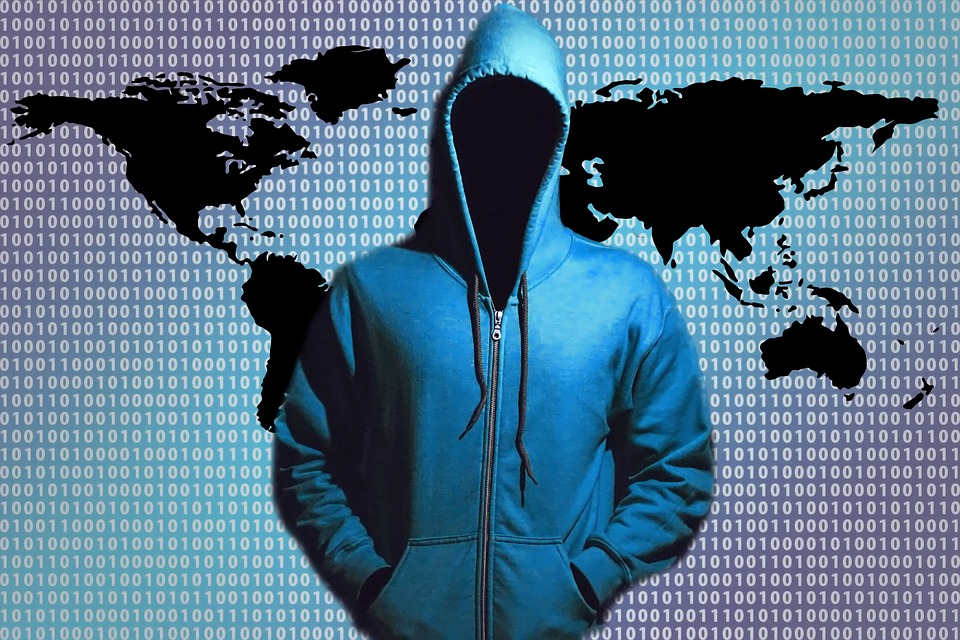
\includegraphics[width=0.8\textwidth]{hacker}
  \end{figure}
  \transdissolve[duration=0.1]
\end{frame}

%%%%%%%%%%%%%%%%%%%%%%%%%%%%%%%%%%%%%%%%%%%%%%%%%%%%%%%%%%%%%%%%%%%%%%%%%%%%%%%%%%%%%%%%%%%%%%%%%%%%%%%%%%%%%%

\section{Presentation of the project}

\subsection{Aim of the project}
\begin{frame}
  \frametitle{Aim of the project}
  \begin{figure}[h]
    \centering
    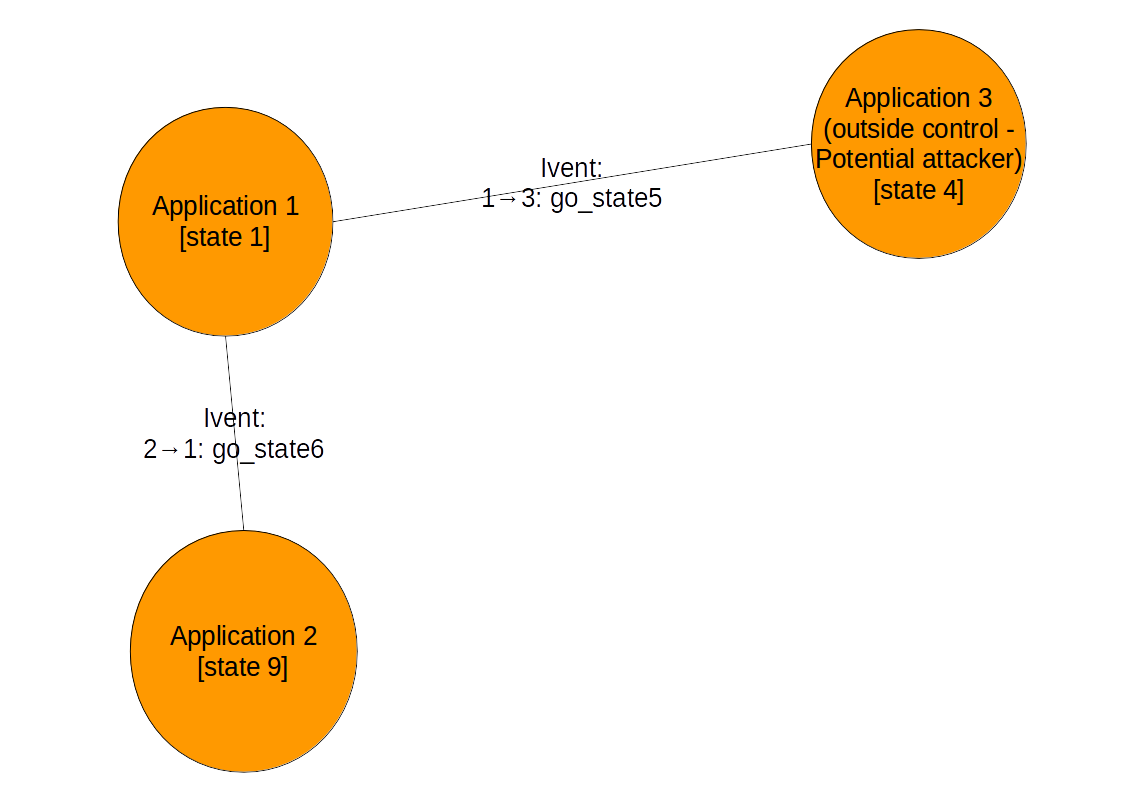
\includegraphics[width=\textwidth]{model}
    \caption{Aim of the project}
  \end{figure}
\transdissolve[duration=0.1]
\end{frame}

\subsection{Technical choices}
\begin{frame}
  \frametitle{Technical choices}%: probes}
  \begin{figure}[h]
    \centering
    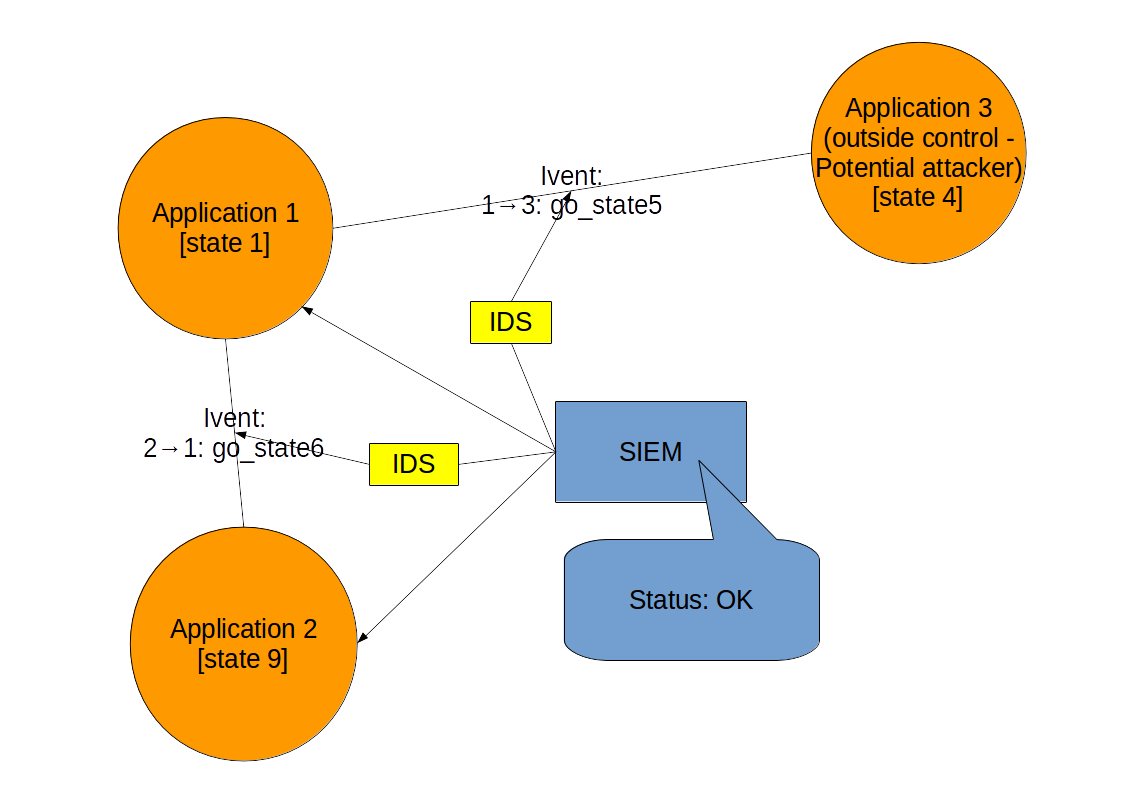
\includegraphics[width=\textwidth]{model_project}
    \caption{Aim of the project}
  \end{figure}
\transdissolve[duration=0.1]
\end{frame}



% \begin{frame}
%   \frametitle{Technical choices: field of study}
%   \begin{figure}[h]
%     \centering
%     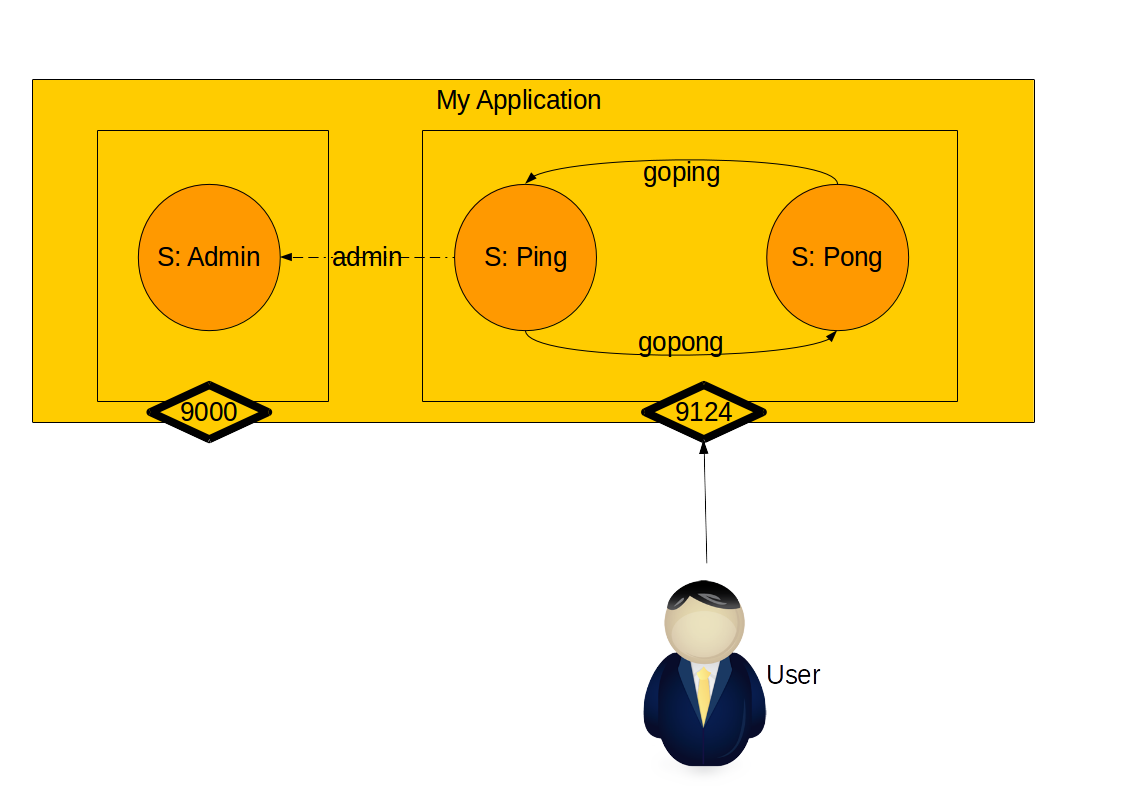
\includegraphics[width=\textwidth]{appli}
%     \caption{Model of the application}
%     \label{fig:model}
%   \end{figure}
% \transdissolve[duration=0.1]
% \end{frame}

\subsection{Organization}
\begin{frame}
  \frametitle{Organization}
  \begin{minipage}[h]{0.45\linewidth}
    \begin{figure}[h]
      \centering
      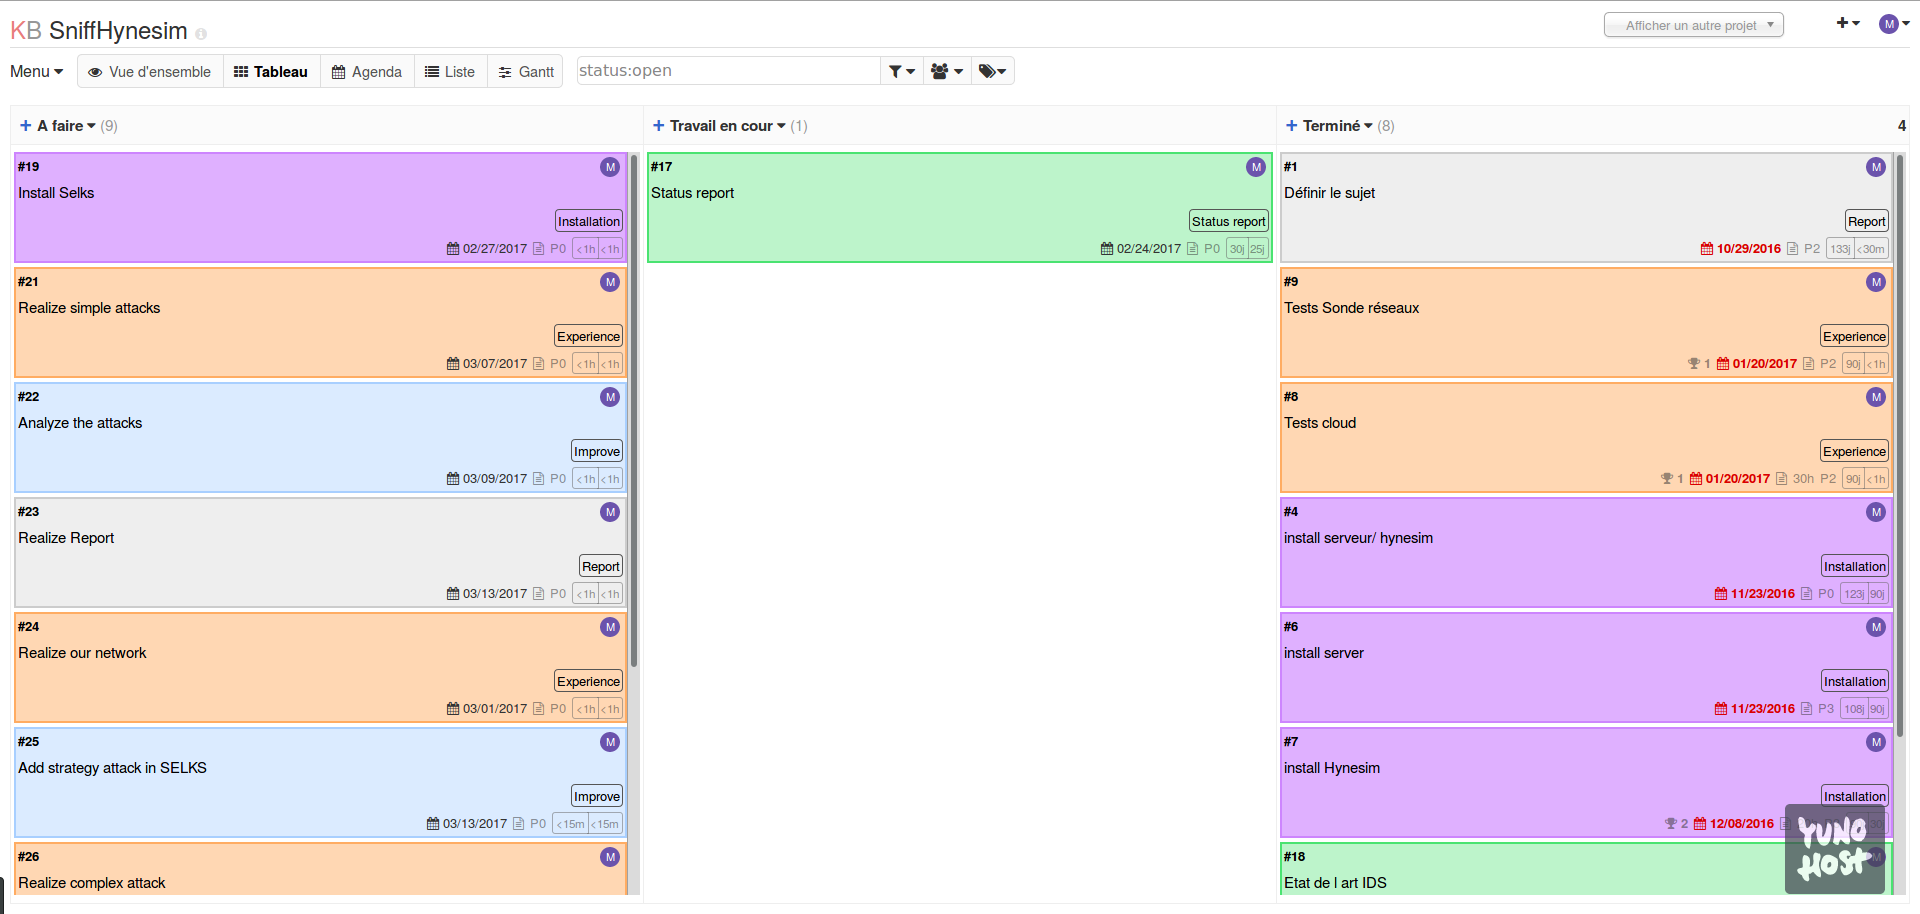
\includegraphics[width=1.2\textwidth]{kandboard}
      \caption{Kanban}
    \end{figure}
  \end{minipage}\hfill
  \begin{minipage}[h]{0.45\linewidth}
    \begin{figure}[h]
      \centering
      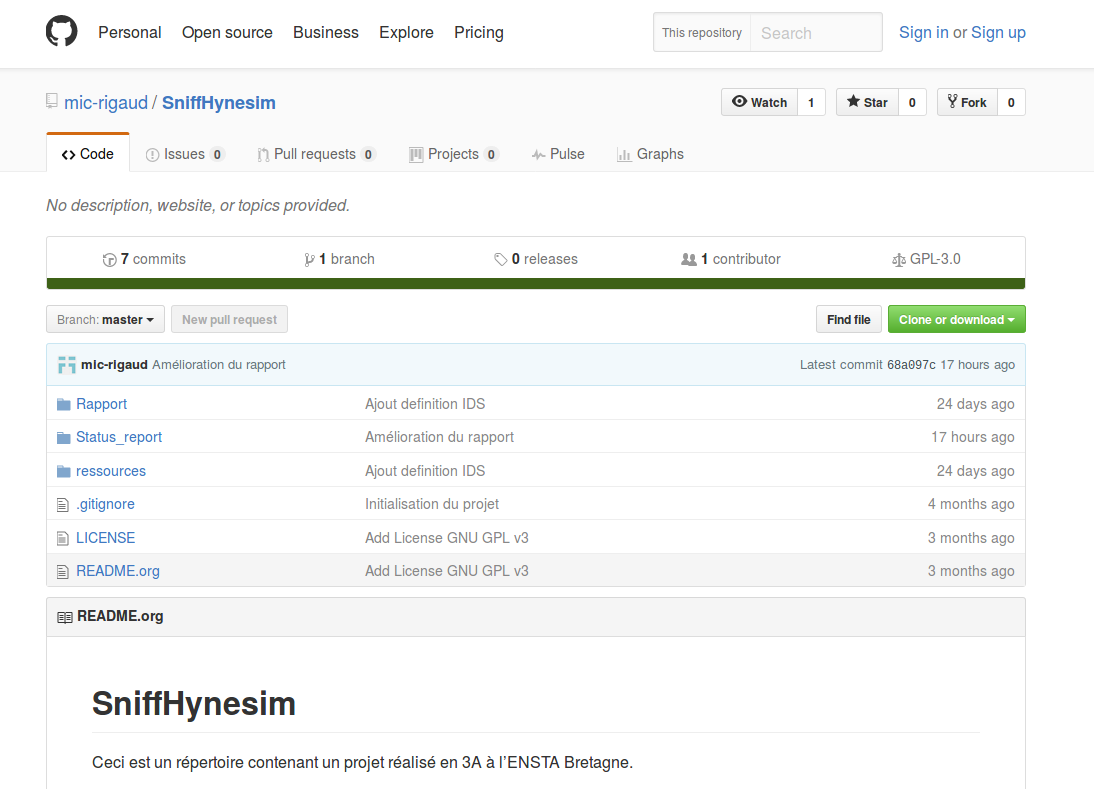
\includegraphics[width=0.8\textwidth]{github}
      \caption{Github}
    \end{figure}
  \end{minipage}
\transdissolve[duration=0.1]
\end{frame}

%%%%%%%%%%%%%%%%%%%%%%%%%%%%%%%%%%%%%%%%%%%%%%%%%%%%%%%%%%%%%%%%%%%%%%%%%%%%%%%%%%%%%%%%%%%%%%%%%%%%%%%%%%%%%%
\section{Technical contribution}

\subsection{Installation}
\begin{frame}
  \frametitle{Installation}
  \begin{figure}[h]
    \centering
    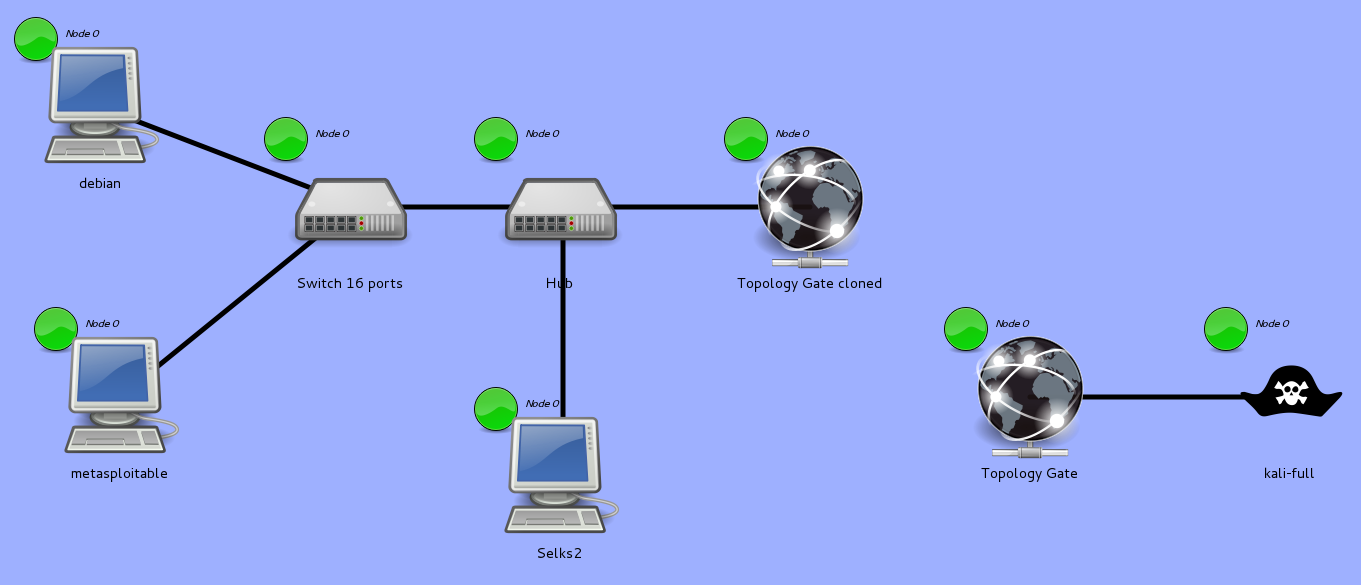
\includegraphics[width=\textwidth]{network_infra}
    \caption{Network installed}
  \end{figure}
\transdissolve[duration=0.1]
\end{frame}

\subsection{Application}
\begin{frame}
  \frametitle{Application}
  \begin{figure}[h]
    \centering
    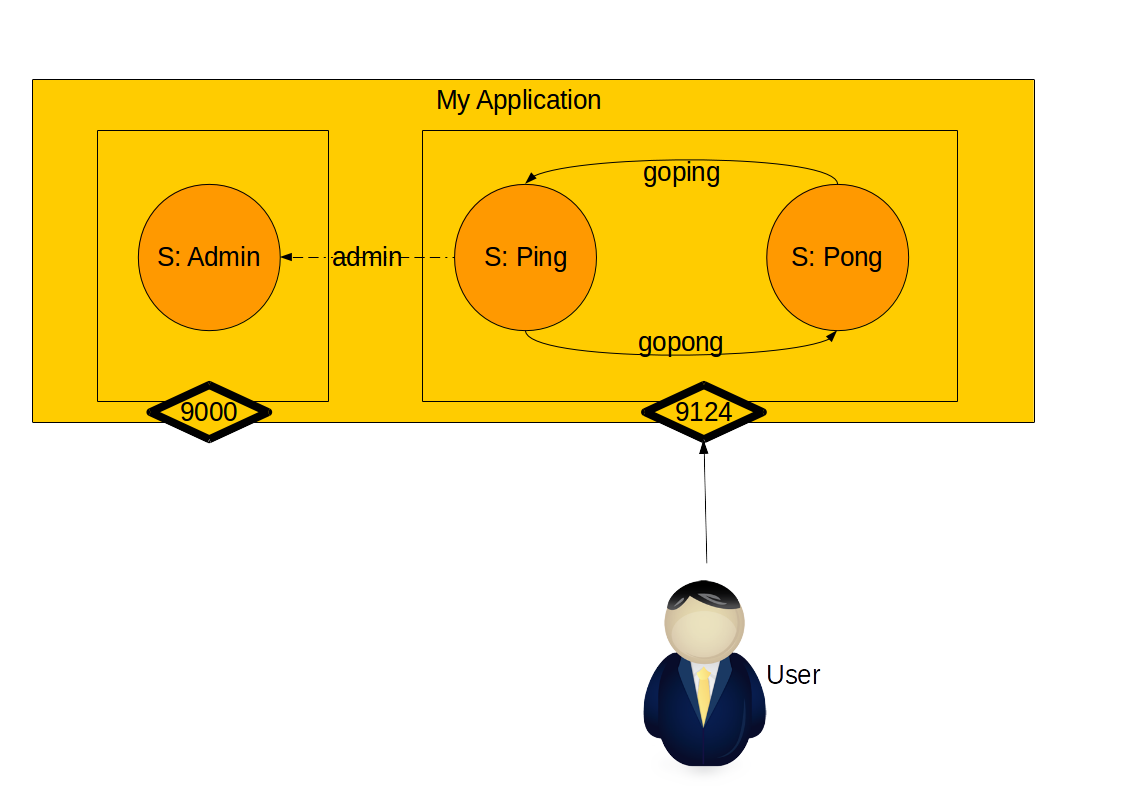
\includegraphics[width=\textwidth]{appli}
    \caption{Model of the application}
    \label{fig:model}
  \end{figure}
\transdissolve[duration=0.1]
\end{frame}


\subsection{Detection system}
\begin{frame}
  \frametitle{Detection system}
  \begin{figure}[h]
    \centering
    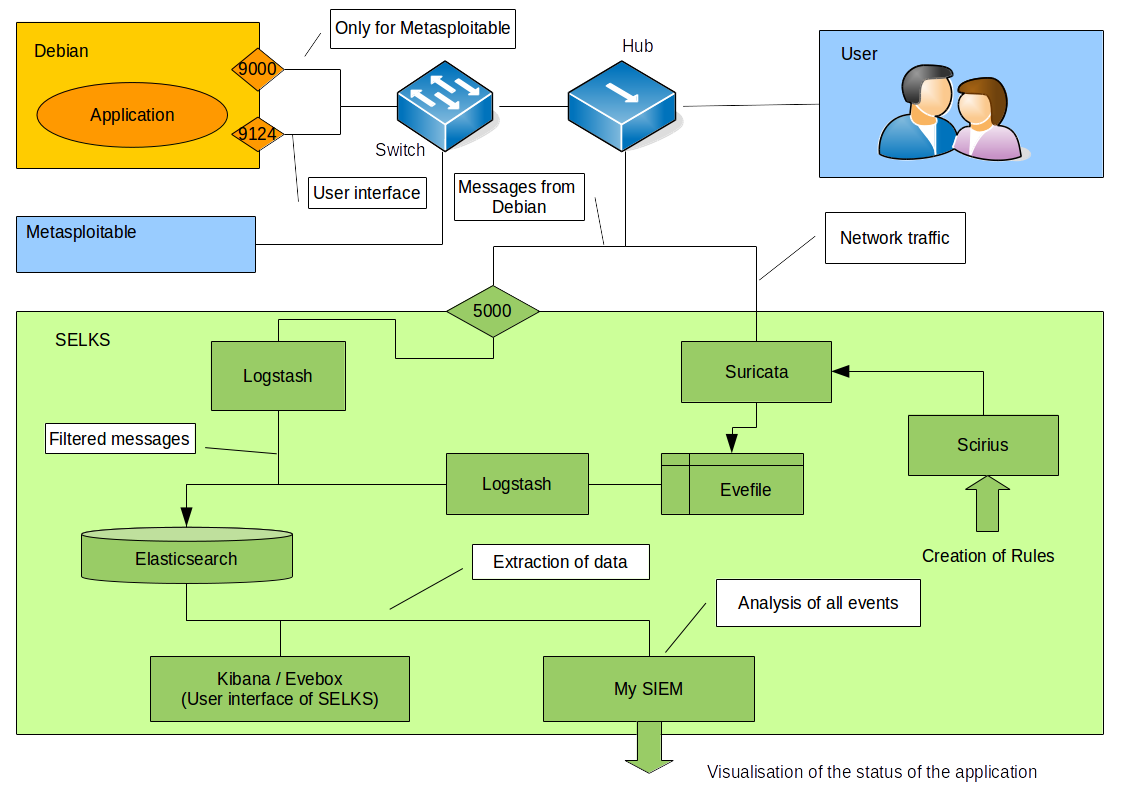
\includegraphics[width=\textwidth]{summary}
    \caption{Summary of the situation}
  \end{figure}
\transdissolve[duration=0.1]
\end{frame}



%%%%%%%%%%%%%%%%%%%%%%%%%%%%%%%%%%%%%%%%%%%%%%%%%%%%%%%%%%%%%%%%%%%%%%%%%%%%%%%%%%%%%%%%%%%%%%%%%%%%%%%%%%%%%%
\section{Results}

\subsection{Results}
\begin{frame}
  \frametitle{Results}

\transdissolve[duration=0.1]
\end{frame}

\subsection{Way of improvements}
\begin{frame}
  \frametitle{Way of improvements}

\transdissolve[duration=0.1]
\end{frame}

%%%%%%%%%%%%%%%%%%%%%%%%%%%%%%%%%%%%%%%%%%%%%%%%%%%%%%%%%%%%%%%%%%%%%%%%%%%%%%%%%%%%%%%%%%%%%%%%%%%%%%%%%%%%%%
\section{Conclusion}
\begin{frame}
  \frametitle{Conclusion}
  \begin{figure}[h]
    \centering
    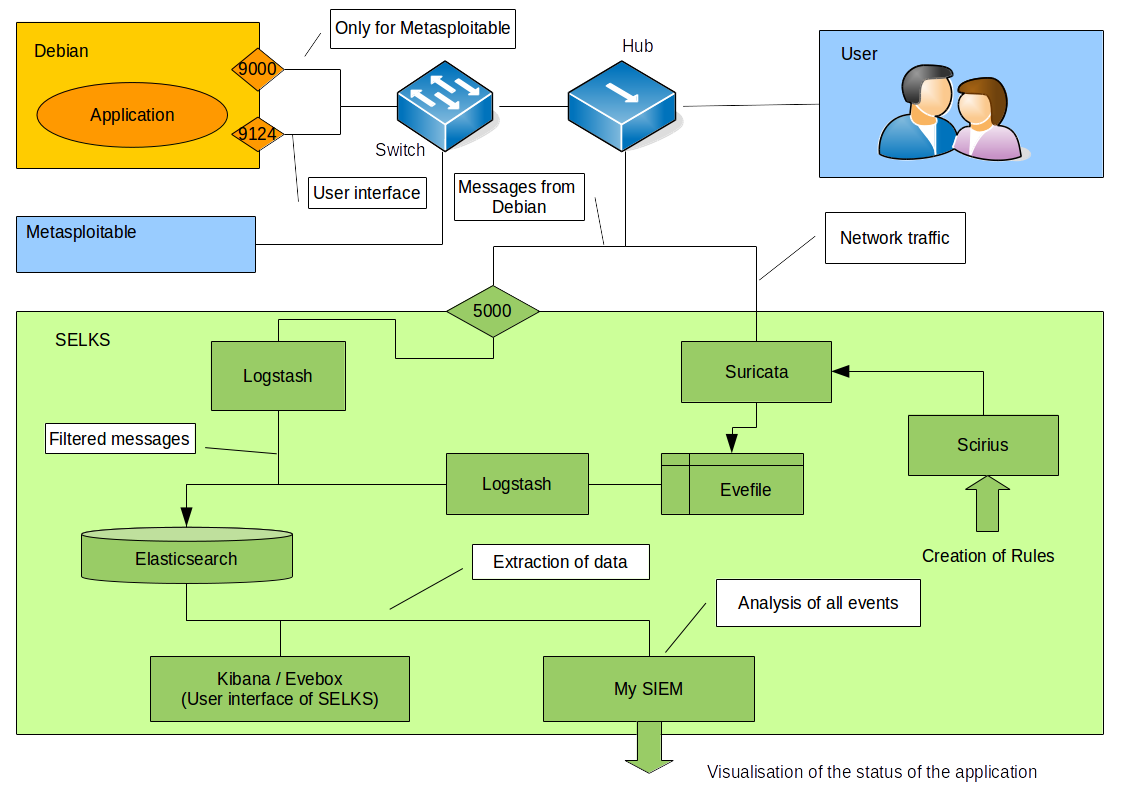
\includegraphics[width=\textwidth]{summary}
    \caption{Summary of the situation}
  \end{figure}
  \transdissolve[duration=0.1]
\end{frame}

\begin{frame}[allowframebreaks]
  \frametitle{Demonstration}
  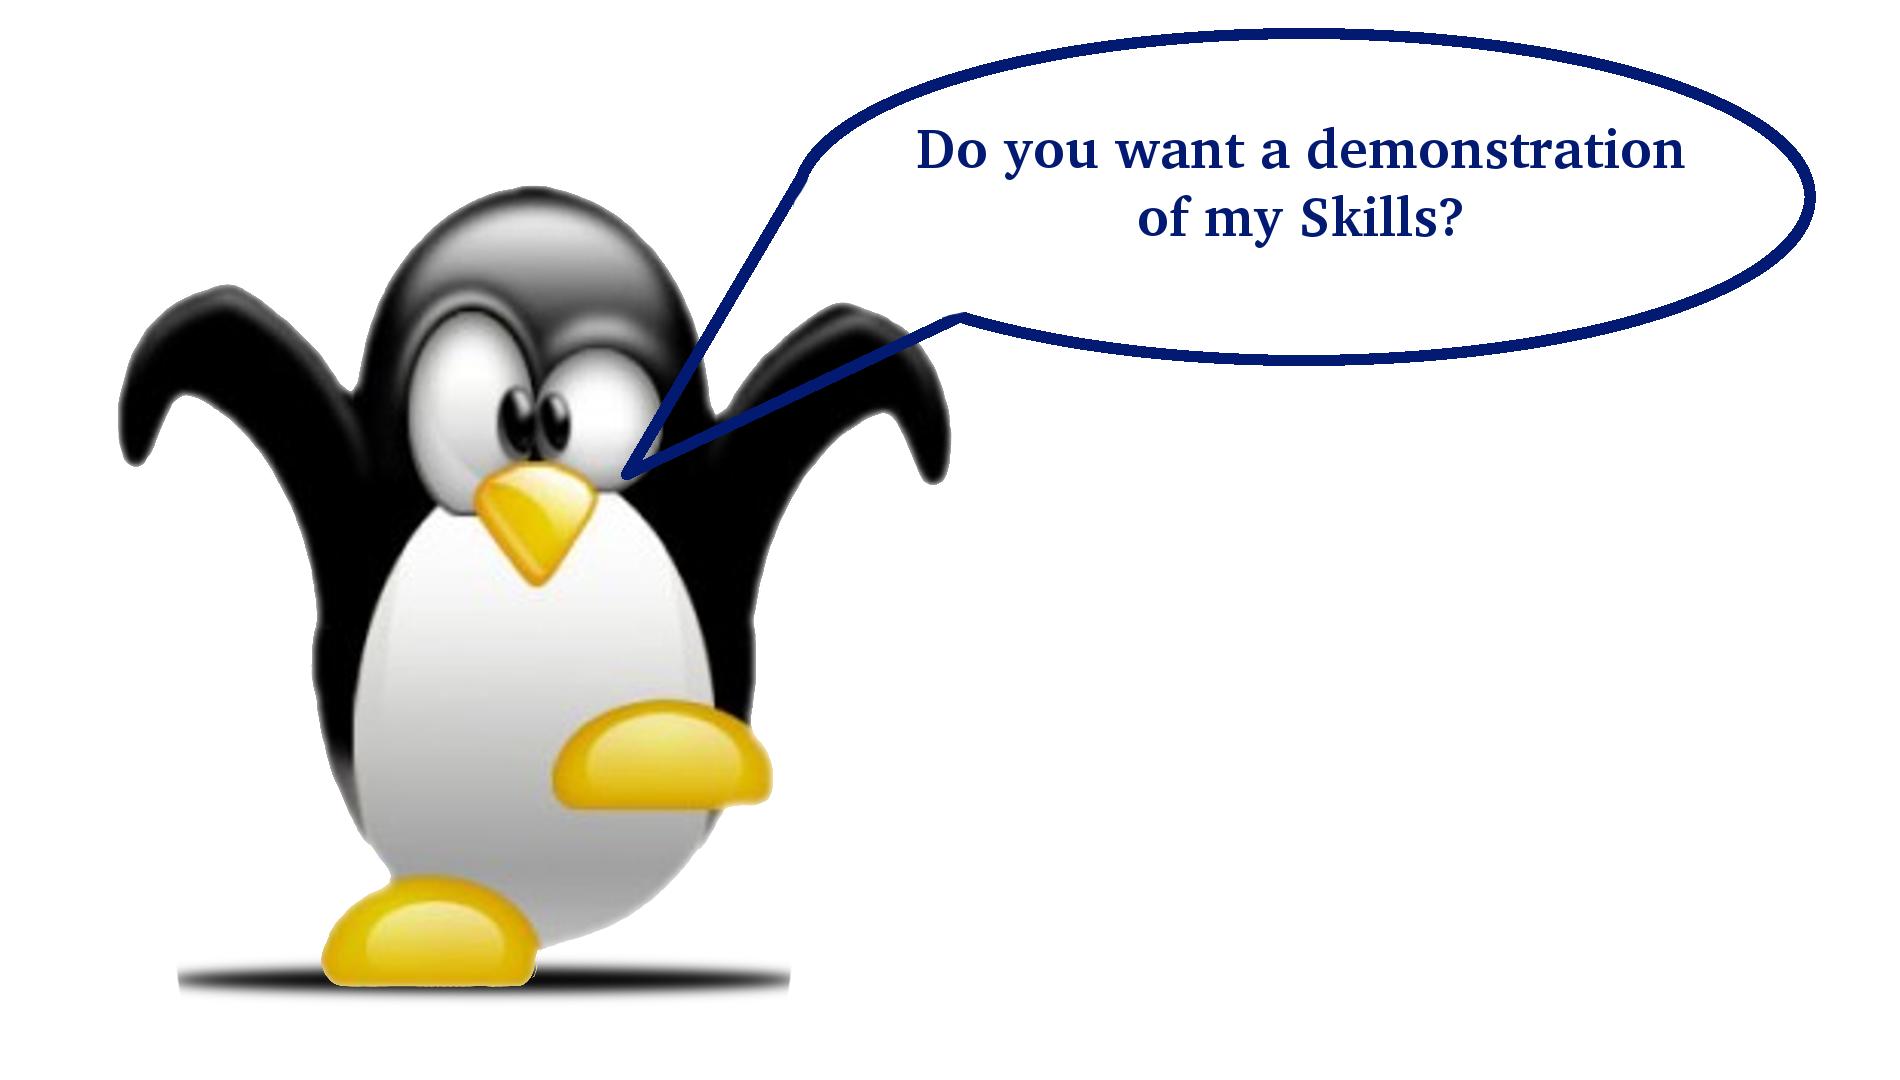
\includegraphics[width=\textwidth]{tux_demo_en}
  \transdissolve[duration=0.1]
\end{frame}

\begin{frame}[allowframebreaks]
  \frametitle{Bibliography}
  \nocite{*}
  \bibliography{biblio}
  \transdissolve[duration=0.1]
\end{frame}


\begin{frame}
  \frametitle{Questions?}

  \begin{center}
    
\includegraphics[width=0.7\textwidth]{tux_ask}
  \end{center}
  \transdissolve[duration=0.1]
\end{frame}

\appendix

\subsection{IDS}
\begin{frame}
  \frametitle{IDS}

  \definitionn{IDS}{An intrusion detection system (IDS) inspects all inbound and outbound network activity and
    identifies suspicious patterns that may indicate a network or system attack from someone attempting to break
    into or compromise a system.}

\transdissolve[duration=0.1]
\end{frame}

\subsection{SIEM}
\begin{frame}
  \frametitle{SIEM}
  \definitionn{SIEM}{In the field of computer security, security information and event management (SIEM) software
    products and services combine security information management (SIM) and security event management (SEM). They
    provide real-time analysis of security alerts generated by network hardware and applications.}
\transdissolve[duration=0.1]
\end{frame}

\subsection{SELKS}
\begin{frame}
  \frametitle{SELKS}
  \begin{figure}[h]
    \centering
    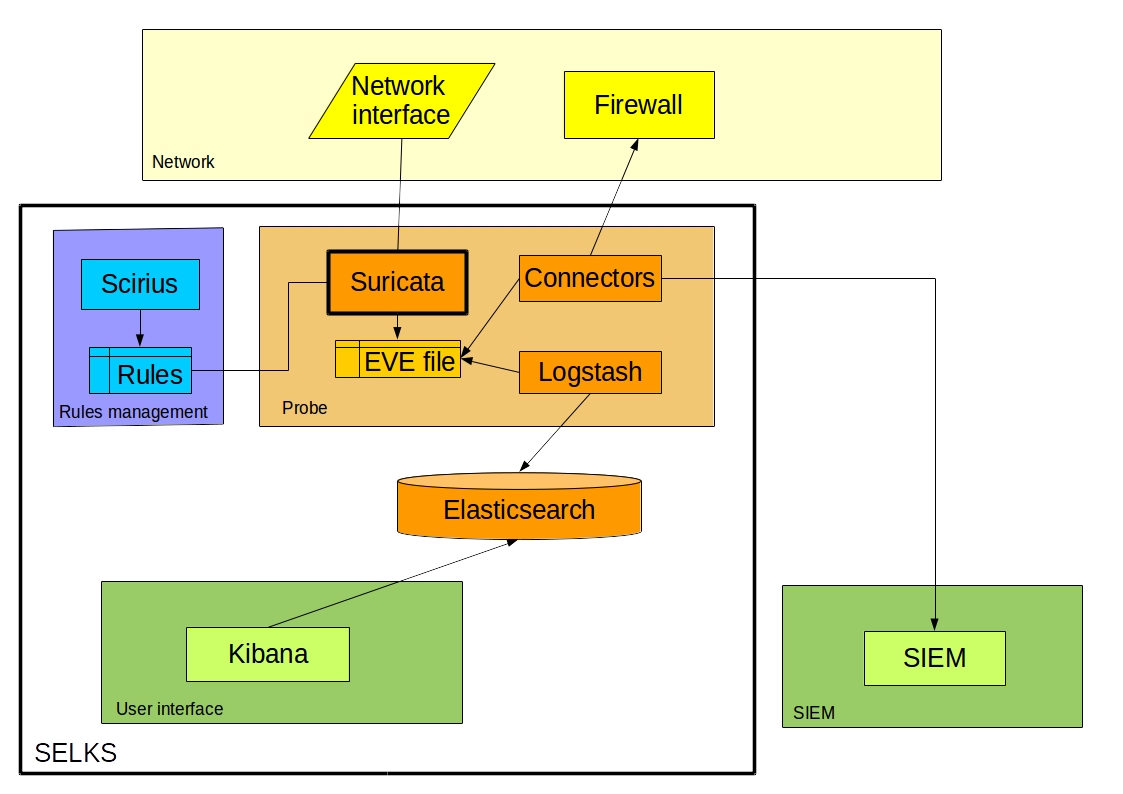
\includegraphics[width=\textwidth]{selks_archi}
    \caption{SELKS}
    \label{fig:selks}
  \end{figure}
\transdissolve[duration=0.1]
\end{frame}

\subsection{Evebox}
\begin{frame}
  \frametitle{Evebox}
  \begin{figure}[h]
    \centering
    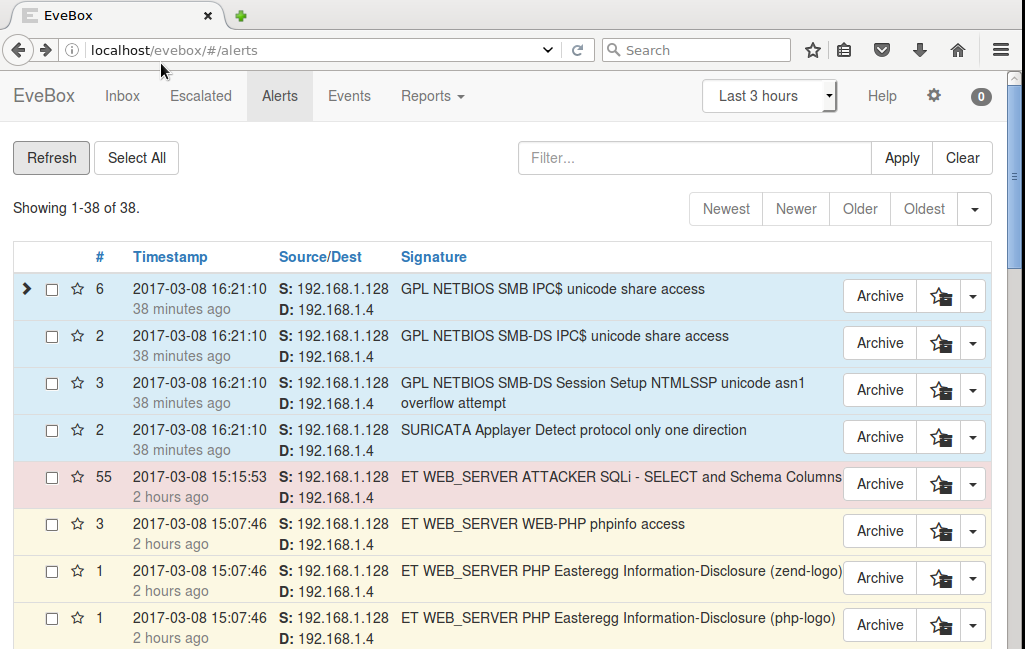
\includegraphics[width=\textwidth]{evebox}
  \end{figure}
\transdissolve[duration=0.1]
\end{frame}

\subsection{Kibana}
\begin{frame}
  \frametitle{Kibana}
  \begin{figure}[h]
    \centering
    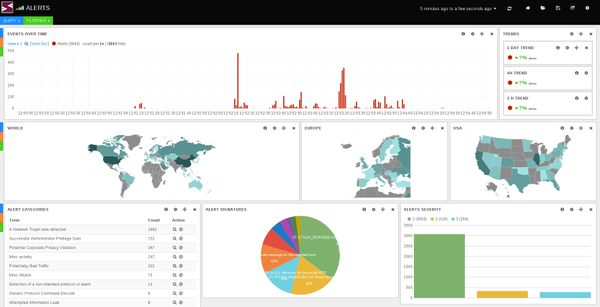
\includegraphics[width=\textwidth]{kibana}
  \end{figure}
\transdissolve[duration=0.1]
\end{frame}

\subsection{IDS rules}
\begin{frame}[fragile]
  \frametitle{IDS rules}
  \scriptsize
  \begin{lstlisting}[language=suricata]
    alert tcp any any -> any 9124 (msg:"Action goping"; \
    content:"goping"; sid:501; rev:5000;)

    alert tcp any any -> any 9124 (msg:"Action gopong"; \
    content:"gopong"; sid:502; rev:5001;)

    alert tcp any any -> any 9000 (msg:"Connexion vers l interface admin"; \
    flow:established,to_server sid:504; rev:5002;)
  \end{lstlisting}
\transdissolve[duration=0.1]
\end{frame}

\subsection{SIEM}
\begin{frame}
  \frametitle{SIEM: Application probe}
  \begin{figure}[h]
    \centering
    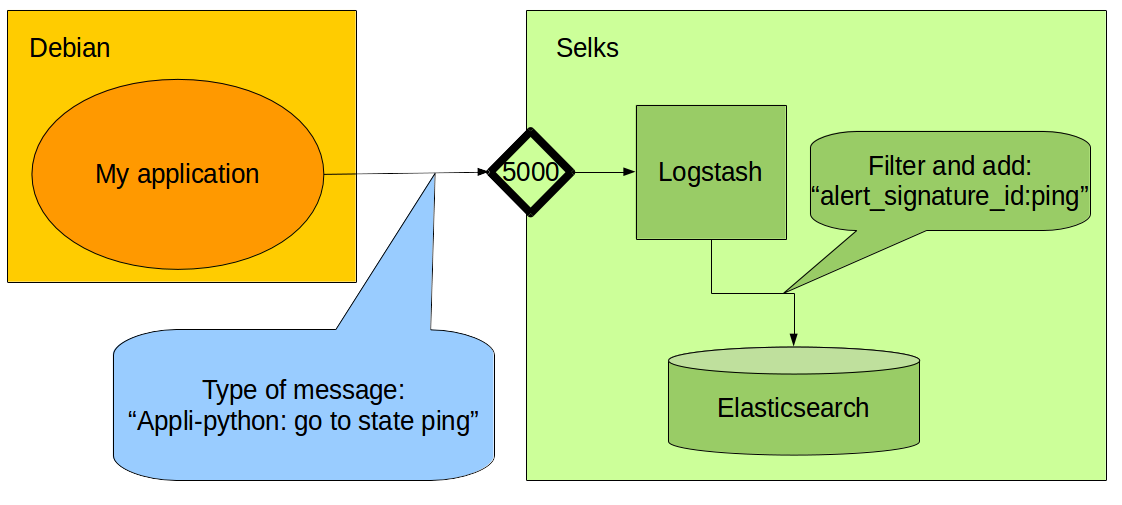
\includegraphics[width=\textwidth]{traitement_donnes}
    \caption{Data processing}
    \label{fig:data}
  \end{figure}
\transdissolve[duration=0.1]
\end{frame}

\begin{frame}
  \frametitle{SIEM: Implementation}
  \begin{figure}[h]
    \centering
    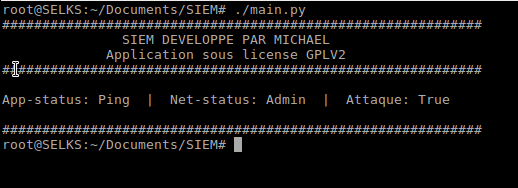
\includegraphics[width=\textwidth]{siem_interface}
    \caption{My SIEM}
  \end{figure}
\transdissolve[duration=0.1]
\end{frame}


\begin{frame}
  \frametitle{Kanban : Definition}
  \definitionn{Kanban}{Kanban is a new technique for managing a software development process in a highly efficient
  way. Kanban underpins Toyota's "just-in-time" (JIT) production system. The kanban system consists of a big board on
  the wall with cards or sticky notes placed in columns with numbers at the top}

\end{frame}

\begin{frame}
  \frametitle{Kanban: kanboard}
  \begin{figure}[h]
    \centering
    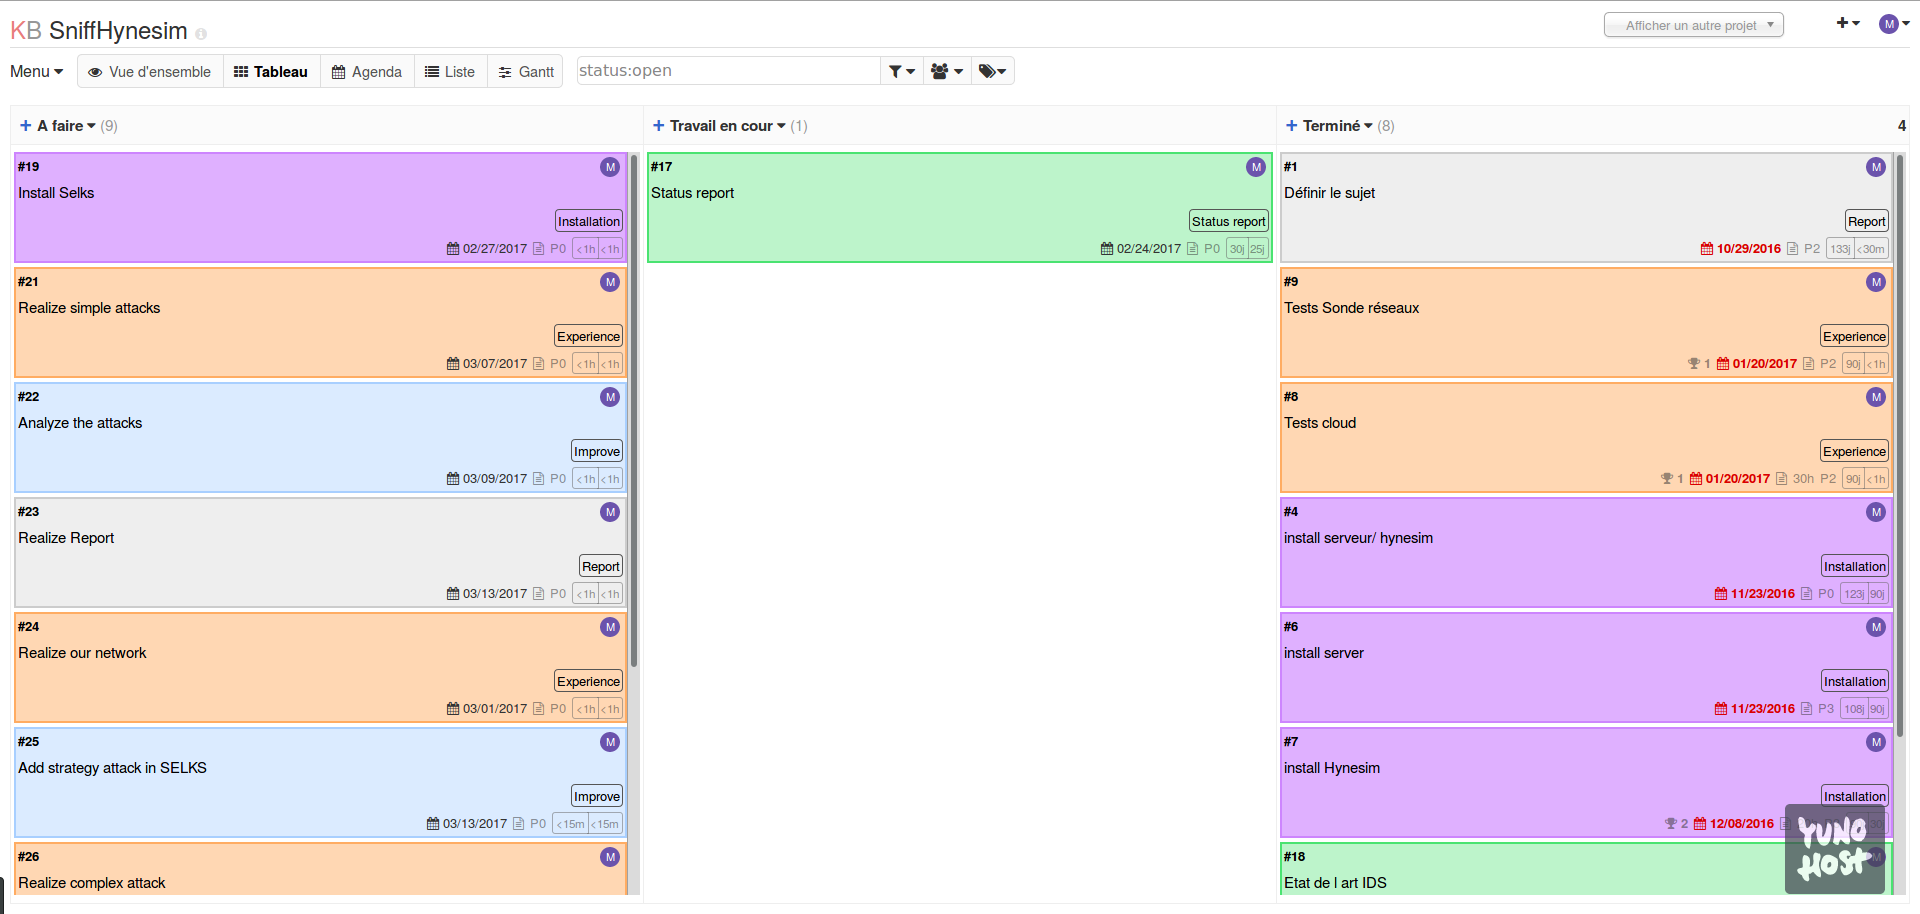
\includegraphics[width=\textwidth]{kandboard}
  \end{figure}
  \url{https://mic-rigaud.fr/kanboard/?controller=BoardViewController&action=readonly&token=10ea65eca908023dbcd8bc8dce75791c7a14d67912627dafaa5b71033222}
\end{frame}

\end{document}


%%% Local Variables:
%%% mode: latex
%%% TeX-master: t
%%% End:
